\documentclass[12pt, a4paper]{article} % 10pt font size (11 and 12 also possible), A4 paper (letterpaper for US letter) and two column layout (remove for one column)


%----------------------------------------------------------------------------------------
%	PACKAGES AND OTHER DOCUMENT CONFIGURATIONS
%----------------------------------------------------------------------------------------

\usepackage[ngerman]{babel} 

%\usepackage{microtype} % Better typography

%\usepackage{amsmath,amsfonts,amsthm} % Math packages for equations

%\usepackage[svgnames]{xcolor} % Enabling colors by their 'svgnames'

\usepackage[hang,small,labelfont=bf,up,textfont=it]{caption} % Custom captions under/above tables and figures

\usepackage{booktabs} % Horizontal rules in tables

\usepackage{graphicx} % Required for adding images
\graphicspath{{figure/}}

\usepackage{enumitem} % Required for customising lists
\setlist{noitemsep} % Remove spacing between bullet/numbered list elements

%\usepackage{sectsty} % Enables custom section titles
%\allsectionsfont{\usefont{OT1}{phv}{b}{n}} % Change the font of all section commands (Helvetica)

\usepackage[hidelinks]{hyperref}

\usepackage{tabularx}

\usepackage[verbose]{placeins}

\usepackage[official]{eurosym}

\usepackage{longtable}

\urlstyle{same}


%----------------------------------------------------------------------------------------
%	MARGINS AND SPACING
%----------------------------------------------------------------------------------------

\usepackage{geometry} % Required for adjusting page dimensions

\geometry{
    head=1cm,
    foot=2cm,
    top=2cm, % Top margin
    bottom=0cm, % Bottom margin
    left=3cm, % Left margin
    right=3cm, % Right margin
    includehead, % Include space for a header
    includefoot, % Include space for a footer
    %showframe, % Uncomment to show how the type block is set on the page
}

\setlength{\columnsep}{7mm} % Column separation width

%----------------------------------------------------------------------------------------
%	FONTS
%----------------------------------------------------------------------------------------

\usepackage[utf8]{inputenc} % Required for inputting international characters
\usepackage[default,osfigures,scale=0.95]{opensans} 
\usepackage[T1]{fontenc}

%----------------------------------------------------------------------------------------
%   TOC	
%----------------------------------------------------------------------------------------
\setcounter{tocdepth}{2}

%----------------------------------------------------------------------------------------
%	HEADERS AND FOOTERS
%----------------------------------------------------------------------------------------

\usepackage{fancyhdr} % Needed to define custom headers/footers
\pagestyle{fancy} % Enables the custom headers/footers

%\renewcommand{\headrulewidth}{0.0pt} % No header rule
%\renewcommand{\footrulewidth}{0.4pt} % Thin footer rule

%\renewcommand{\sectionmark}[1]{\markboth{#1}{}} % Removes the section number from the header when \leftmark is used

%\nouppercase\leftmark % Add this to one of the lines below if you want a section title in the header/footer

% Headers
\lhead{} % Left header

% Footers
%\lfoot{} % Left footer
%\cfoot{} % Center footer
%\rfoot{\footnotesize\thepage} % Right footer, "Page 1 of 2"

%\fancypagestyle{firstpage}{ % Page style for the first page with the title
%\fancyhf{}
%\renewcommand{\footrulewidth}{0pt} % Suppress footer rule
%}

%----------------------------------------------------------------------------------------
%	TITLE SECTION
%----------------------------------------------------------------------------------------


%\newcommand{\authorstyle}[1]{{\large\usefont{OT1}{phv}{b}{n}\color{Black}#1}} % Authors style (Helvetica)

 


\usepackage{titling} % Allows custom title configuration

\newcommand{\HorRule}{\rule{\linewidth}{1pt}} % Defines the horizontal rule around the title


\pretitle{
    \vspace{60pt} % Move the entire title section up
    \hspace{310pt}
    \\
    \\
    \vspace{40pt}
    \HorRule\vspace{10pt} % Horizontal rule before the title
    \centering\Huge\textbf
}

\posttitle{\par\vskip 15pt} % Whitespace under the title

\preauthor{} % Anything that will appear before \author is printed

\postauthor{ % Anything that will appear after \author is printed
    \vspace{10pt} % Space before the rule
    \par\HorRule % Horizontal rule after the title
    \vspace{150pt} % Space after the title section
}

\usepackage{xcolor}
\definecolor{df}{HTML}{b5dc17}
\usepackage{tikz}


\usepackage{eso-pic}
\newcommand\BackgroundPic{%
    \put(0,0){%
        \parbox[b][\paperheight]{\paperwidth}{%
            
\includegraphics[width=\paperwidth,height=\paperheight,%
            keepaspectratio]{title_background.pdf}%
        }}}


\fancyfootoffset[L]{\dimexpr\oddsidemargin+1in\relax}
\newcommand*\rect[1]{\begin{tikzpicture}[remember picture,overlay]\fill[df] (0,0) rectangle
        (\paperwidth,\headheight);\node at (0,0.5) {#1};\end{tikzpicture}}

\fancyfoot[L]{\rect{}}
\fancyfoot[C]{\rect{}}
\fancyfoot[R]{\rect{\thepage}}
%----------------------------------------------------------------------------------------
%	ABSTRACT
%----------------------------------------------------------------------------------------

\usepackage{lettrine} % Package to accentuate the first letter of the text (lettrine)
\usepackage{fix-cm}	% Fixes the height of the lettrine

\newcommand{\initial}[1]{ % Defines the command and style for the lettrine
    \lettrine[lines=3,findent=4pt,nindent=0pt]{% Lettrine takes up 3 lines, the text to the right of it is indented 4pt and further indenting of lines 2+ is stopped
        {#1}% The letter
    }{}%
}

\usepackage{xstring} % Required for string manipulation

\newcommand{\lettrineabstract}[1]{
    \StrLeft{#1}{1}[\firstletter] % Capture the first letter of the abstract for the lettrine
    \initial{\firstletter}\textbf{\StrGobbleLeft{#1}{1}} % Print the abstract with the first letter as a lettrine and the rest in bold
}

%----------------------------------------------------------------------------------------
%	BIBLIOGRAPHY
%----------------------------------------------------------------------------------------

%\usepackage[backend=bibtex,style=authoryear,natbib=true]{biblatex} % Use the bibtex backend with the authoryear citation style (which resembles APA)

%\addbibresource{example.bib} % The filename of the bibliography

\usepackage[autostyle=true]{csquotes} % Required to generate language-dependent quotes in the bibliography




\pretolerance=10000 % https://tex.stackexchange.com/questions/31301/how-to-reduce-the-number-of-hyphenation

 % Specifies the document structure and loads requires packages

\renewcommand\thepart{\Alph{part}}

%----------------------------------------------------------------------------------------
%	ARTICLE INFORMATION
%----------------------------------------------------------------------------------------

\begin{document}

\title{ 
Tür an Tür - Digital Factory gGmbH\\
Wirkungsbericht 2018\\
} % The article title

\AddToShipoutPicture*{\BackgroundPic}

\date{} 

\maketitle


%----------------------------------------------------------------------------------------
%	ABSTRACT
%----------------------------------------------------------------------------------------

%\lettrineabstract{ }

%----------------------------------------------------------------------------------------
%	ARTICLE CONTENTS
%----------------------------------------------------------------------------------------

\newpage
\tableofcontents

\newpage
\section*{Vorwort}
\addcontentsline{toc}{section}{Vorwort}

Liebe Freunde, Förderer und Begleiter von Integreat, \\ \\
in Ihren Händen halten Sie unseren Wirkungsbericht für das Jahr 2016. Angefangen hat unsere Geschichte mit einer Broschüre für Zuwanderer in Augsburg aus dem Jahr 1997. Anfang 2015 schmiedeten wir gemeinsam mit der Stadt und Initiativen den Plan eben jenen lokalen Alltagshelfer zu digitalisieren. Nach der ersten Analyse von Zielgruppe, IT-Nutzungsverhalten und Prozessen zur Informationsgewinnung und -übersetzung stand die Entscheidung fest: kollaborativ und digital muss die Lösung sein. Gemeinsam mit der TU München entwickelten wir ehrenamtlich die Integreat-App und das zugehörige Verwaltungssystem. Im November 2015 folgte der Start in Augsburg, ehe viele weitere Städte und Landkreise ebenfalls aufsprangen. Mittlerweile umfasst unser Team fast 40 aktive Ehrenamtliche und Integreat bewirkt mehr als wir am Anfang gedacht hätten. Mehrsprachige Informationen bereitzustellen ist keine Mammutaufgabe mehr, als Neuzugewanderte auf lokale Informationen zuzugreifen geht jederzeit auch ohne Internet und Behörden begreifen die Digitalisierung als Chance. Dies sind nur drei der Punkte, die wir mit Integreat erreicht haben.
Wo am Anfang noch Erstinformationen zur Orientierung im Fokus standen, sprechen wir nun über vier Themenbereiche der Integration: Arbeitsmarktzugang, Sprachlernförderung, Wohnen und Partizipation. Die Bedürfnisse ändern sich kontinuierlich, doch wir versuchen unsere Zielgruppe bestmöglich zu kennen. Dazu gehört nicht nur die Tatsache, dass unser Projektteam diversifiziert aufgestellt ist und unser Unternehmenssitz in einem Café für Geflüchtete ist, sondern auch die enge Kooperation mit Asylsozialberatungen und der Wohlfahrt, die uns mit Rat und Tat zur Seite stehen. 
Integreat ist mehr als „nur eine App“ und soll die Städte und Landkreise in Deutschland nachhaltig bei Herausforderungen der Migration und Integration unterstützen. In unserem Wirkungsbericht zeigen wir Ihnen, mit welchen Ressourcen und Aktivitäten wir langfristig Veränderungen schaffen. \\

In diesem Sinne viel Spaß beim Lesen, \\

\noindent \begin{flushleft}
\begin{tabular}{l}
 
\includegraphics[height=1.2cm]{signature.png}\tabularnewline
Daniel Kehne, Projektkoordinator\tabularnewline
\end{tabular}
\par\end{flushleft}

\newpage
\part{Überblick}
\section{Einleitung}
\subsection{Vision und Ansatz}

Die Tür an Tür - Digital Factory gGmbH (nachfolgend Tür an Tür - Digitalfabrik genannt) wurde im Sommer 2016 mit dem Ziel gegründet, Geflüchteten den Einstieg in die neue Gesellschaft zu erleichtern. Um sich in einer neuen Umgebung zurecht zu finden, ist es für die Menschen wichtig, sich einen Überblick über die Angebote, Gesetze und Ansprechpartner vor Ort zu verschaffen. Durch verschiedene Angebote stehen den Geflüchteten generelle Informationen über das Leben in Deutschland zur Verfügung. Es mangelt bereits jedoch an lokalen Informationsangeboten, da diese, wenn überhaupt, nur in deutscher Sprache verschriftlicht sind. Derartige Informationsdefizite auszugleichen, ist der Tür an Tür - Digitalfabrik ein großes Anliegen und wir hoffen dieses Ziel durch unsere gesamten Aktivitäten -  insbesondere jedoch durch die App Integreat -  zu erreichen. Langfristig soll Integreat als ständiger Integrationsbegleiter und digitaler Buddy verstanden werden und nicht nur Erstinformationen, sondern auch andere hilfreiche Funktionen zum Leben in der eigenen Kommune bieten. 
Die Tür an Tür - Digitalfabrik steht nicht nur für praktische Geflüchtetenhilfe, sondern auch für den Fortschritt des E-Governments. Durch unser auf die Ansprüche unserer kommunalen Kooperationspartner abgestimmtes Angebot führen wir Behörden schrittweise an die Möglichkeiten der Digitalisierung heran und öffnen dadurch die Tür für weitere Entwicklungen in diese Richtung. 
Integreat als mobiler Flüchtlingsguide ist das Flaggschiff der Digitalfabrik. Das Angebot der gemeinnützigen Organisation soll in Zukunft jedoch durch weitere Projekte ergänzt werden. Da diesbezügliche Projekte erst für das Jahr 2017 in Planung sind, wird sich dieser Bericht hauptsächlich auf Integreat fokussieren. Geplante Projekte sind unter Teil 7.3 angeführt.

\newpage
\subsection{Gegenstand des Berichts}

\begin{table}[!h]
\centering
\label{table1}
\begin{tabular}{|p{4cm}|p{10 cm}|}
\hline
Geltungsbereich                     & Dieser Bericht bezieht sich auf die Aktivitäten der Tür an Tür - Digital Factory gGmbH. Ein besonderer Fokus wird auf das Kernprodukt Integreat gelegt.\\ \hline
Berichtszeitraum und Berichtszyklus & Wir berichten über unsere Arbeit im Jahr 2016 ab Beginn der Gründung am 22.06.2016. An einigen Stellen fließen Aktivitäten ab dem Jahr 2015 vor der Gründung mit ein.\\ \cline{1-2}
Anwendung des SRS                   & In diesem Bericht orientieren wir uns stark an den Vorgaben der aktuellen Version des Social Reporting Standards (SRS), Stand 2014. Dies ist der erste Jahresbericht nach dem SRS.\\ \cline{1-2} \hline
Ansprechpartnerin                     & Clara Bracklo \href{mailto:bracklo@integreat-app.de}{bracklo@integreat-app.de}\\ \hline
\end{tabular}
\end{table}


\begin{figure} [!h]
    \centering
	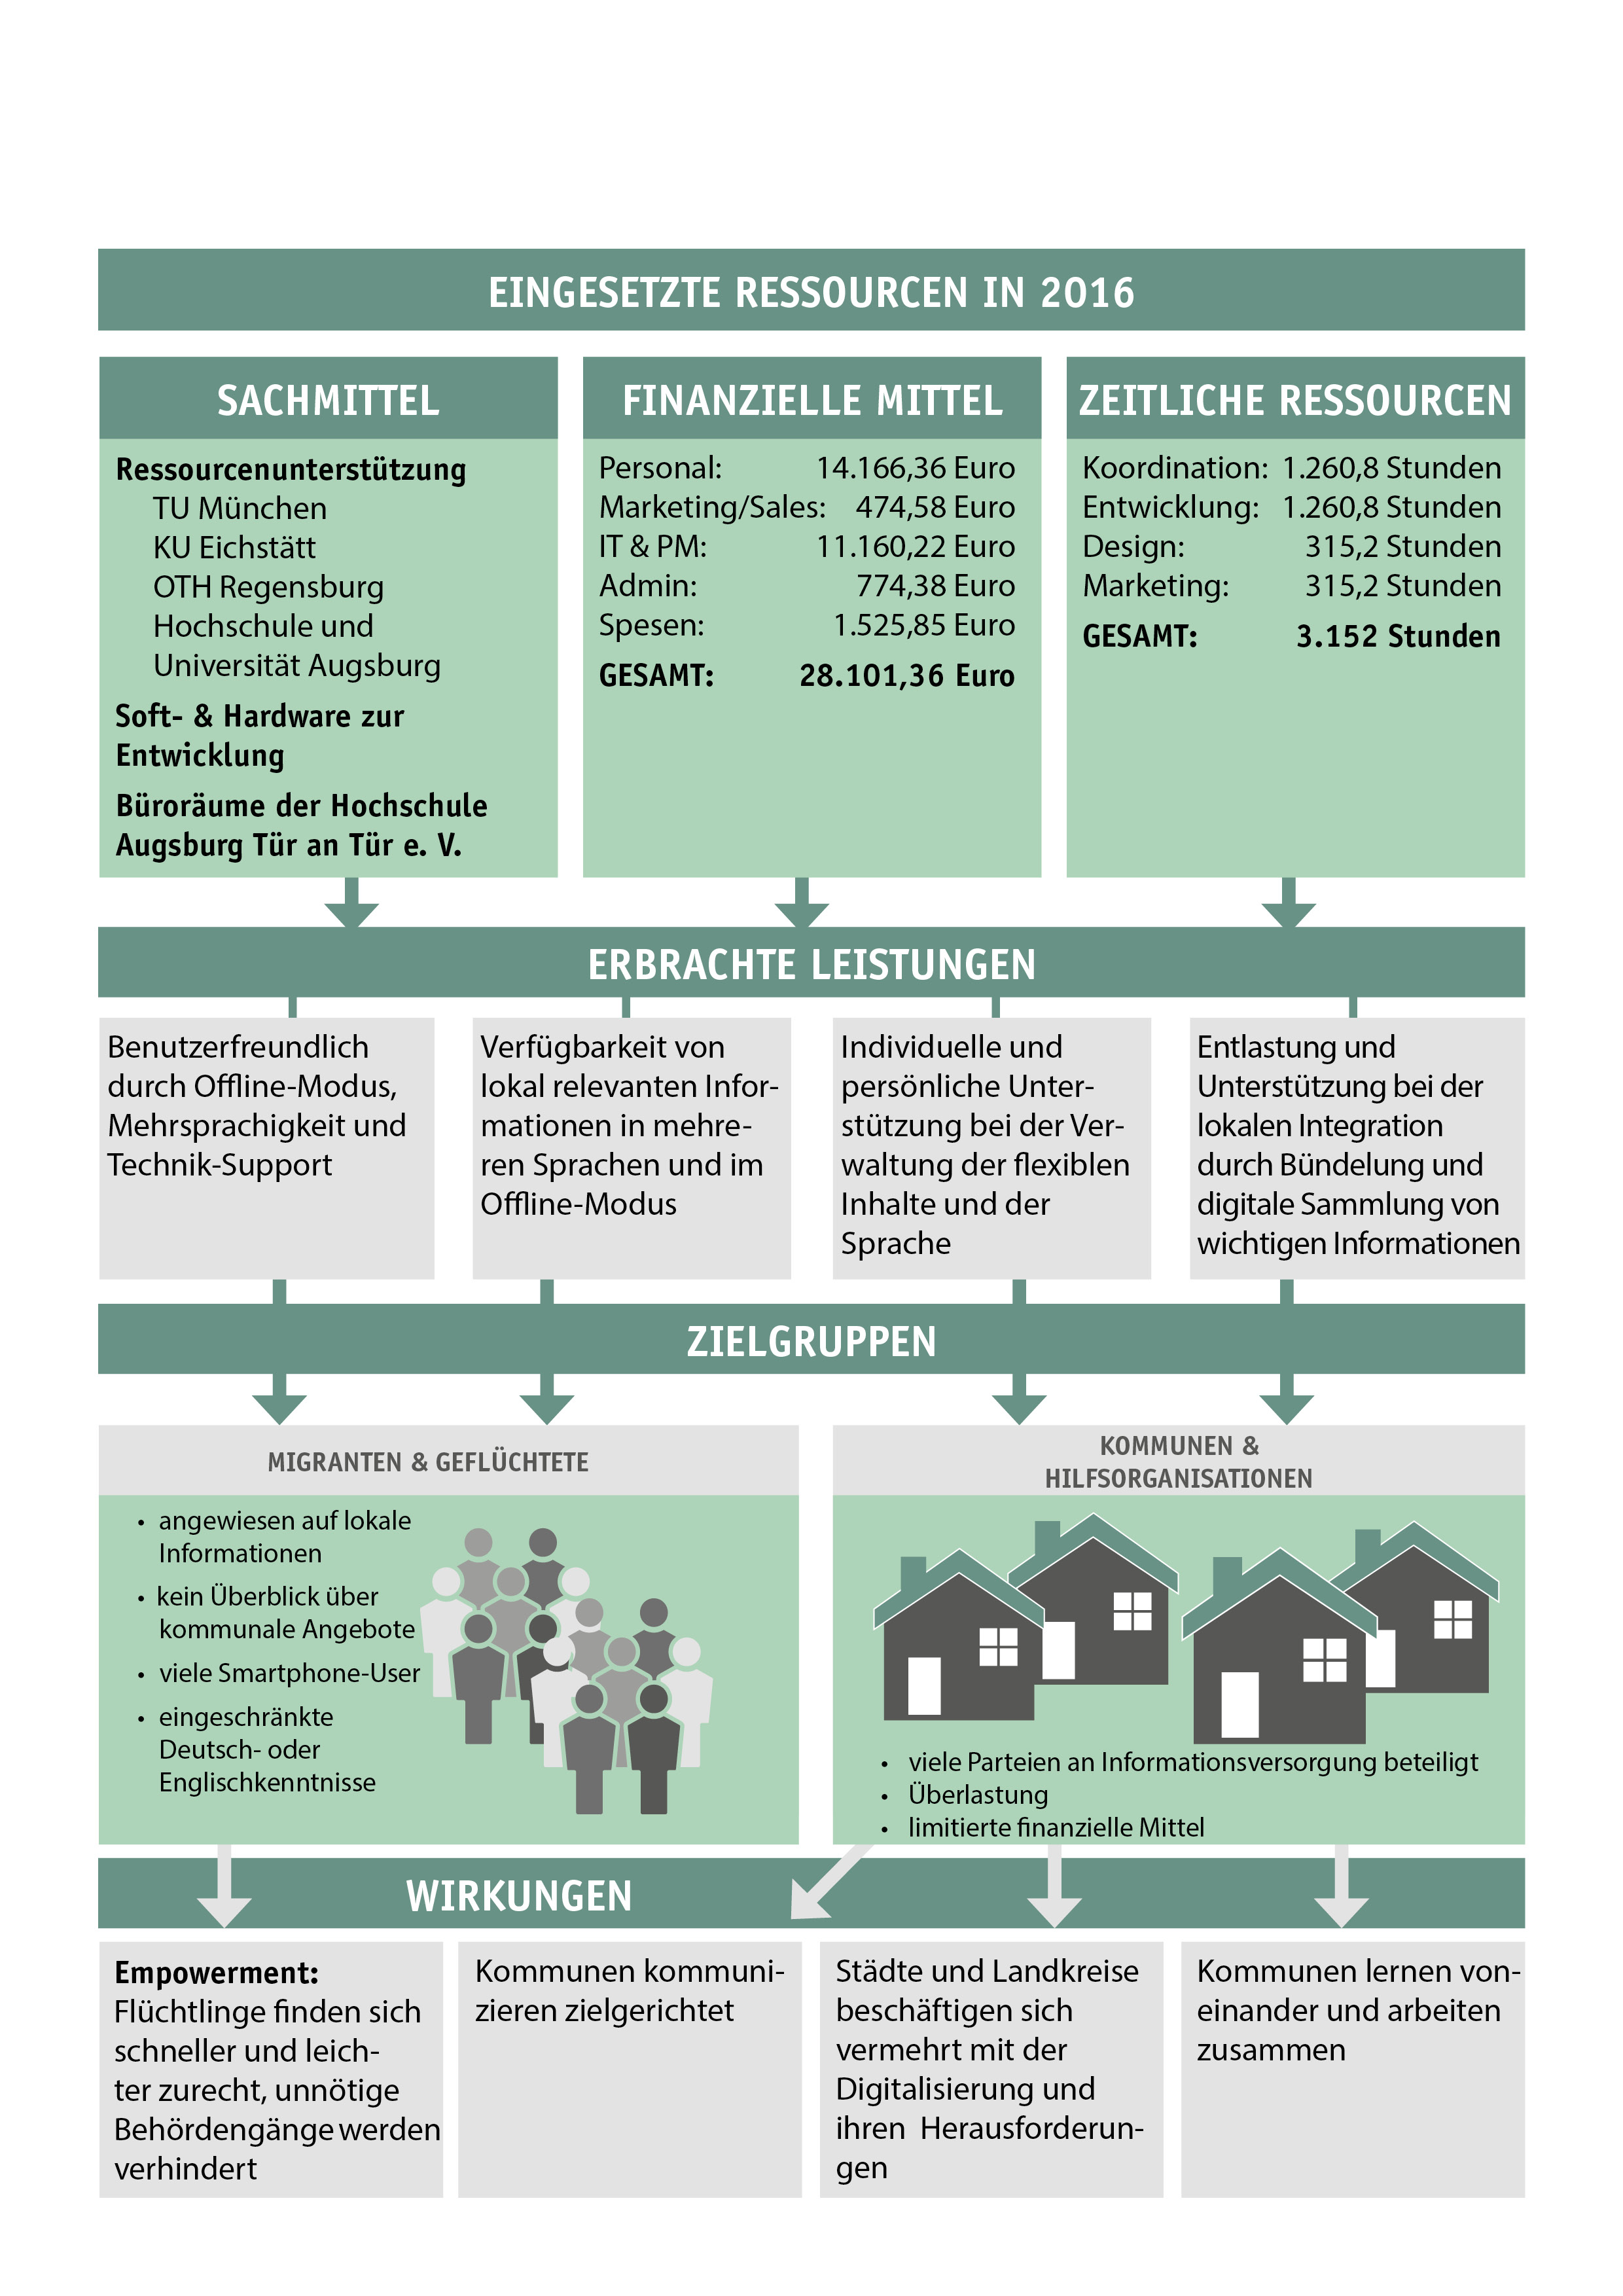
\includegraphics[width=14cm]{wirkungskette_neu.jpg} % Figure image
	\caption{Wirkungskette} % Figure caption
	\label{fig:wirkungskette} % Label for referencing with \ref{bear}
\end{figure}

\part{Die Organisation}
\section{Organisationsprofil}
\subsection{Allgemeine Angaben}

\begin{table}[!h]
\centering
\label{table1}
\begin{tabular}{|p{5cm}|p{9 cm}|}
\hline
Name                     & Tür an Tür – Digital Factory gGmbH\\ \hline
Sitz der Organisation gemäß Satzung                    & Augsburg\\ \hline
Gründung                     & 22.06.2016\\ \hline
Rechtsform                     & gGmbH\\ \hline
Kontaktdaten                     & Wertachstr. 29\\ 
Adresse                    & 86153 Augsburg\\ 
Telefon                   & +49 (0) 821/90799-0\\
E-Mail                    & \href{mailto:info@integreat-app.de}{info@integreat-app.de}\\
Website (URL)                  & \url{http://integreat-app.de}\\
\hline
Link zur Satzung (URL)                   & \url{http://tuerantuer.de/wp-content/uploads/2017/05/Gesellschaftsvertrag_TATDF_final.pdf }\\ \hline
Registergericht                    & Finanzamt Augsburg-Stadt\\ 
Registernummer                   & HRB30759\\ 
Datum der Eintragung                  & 03.05.2016\\ \hline
Angabe über Gemeinnützigkeit gemäß §52 Abgabenordnung                    &  Gemeinnützigkeit gemäß §52 Abgabenordnung festgestellt am 13.09.2016 vom Finanzamt Augsburg-Stadt\\ 
Datum des Feststellungsbescheids                   &   \\ 
Ausstellendes Finanzamt                  & \\ 
Erklärung des gemeinnützigen Zwecks     & Gemeinnützige Zwecke sind laut Satzung: Internationale Gesinnung, Toleranz auf allen Gebieten der Kultur und des Völkerverständigungsgedanken, Hilfe für politisch, rassisch oder religiös Verfolgte, für Flüchtlinge und Vertriebene\\ \hline
Anzahl MitarbeiterInnen                    & 41\\ 
davon hauptamtlich                    & 5\\ 
davon Honorarkräfte                     & 0\\ 
davon ehrenamtlich                  & 36\\ \hline
\end{tabular}
\end{table}

\subsection{Einnahmen und Ausgaben}

\begin{table}[!h]
\centering
\label{table1}
\begin{tabular}{|p{6cm}|p{8 cm}|}
\hline
Währung, Einheit                    & Euro, \euro{}\\ \hline
\textbf{Einnahmen}                  & \\ \hline
1. Erlöse                    & 5.750,00\\ \hline
davon aus öffentlichen Aufträgen   & 0,00\\ \hline
2. Zuwendungen                     & 22.763,63\\ \hline
davon aus öffentlicher Hand (Zuschüsse)                    & 22.763,63\\ \hline
3. Beiträge    & 0,00\\ \hline
4. Sonstige Einnahmen (Preisgelder, Spenden)                     & 4.800,00\\ \hline
\textbf{Summe Einnahmen}                 & \textbf{33313,63}\\ \hline
& \\ \hline
\textbf{Ausgaben (wenn Sie 500.000 Euro oder mehr Gesamteinnahmen haben)}&   \\ \hline
A1. Projektkosten
            & \\ \hline
A2. Werbekosten           & \\ \hline
A3. Verwaltungskosten              & \\ \hline
4. Finanzierungskosten             & \\ \hline
5. Steuern             & \\ \hline
6. Sonstige Ausgaben             & \\ \hline
\textbf{Summe Ausgaben}                 & \\ \hline

& \\ \hline
\textbf{ 
Ausgaben (wenn Sie weniger als 500.000 Euro Gesamteinnahmen haben)}&   \\ \hline
B1. Personalkosten
            & 14.166,36\\ \hline
B2. Sachkosten           & 13.931,67\\ \hline
4. Finanzierungskosten              & 0,00\\ \hline
5. Steuern             & 0,00\\ \hline
6. Sonstige Ausgaben             & 0,00\\ \hline
\textbf{Summe Ausgaben}                 & \textbf{28.098,03}\\ \hline

& \\ \hline
\textbf{ 
Jahresergebnis (Einnahme abzgl. Ausgaben)}& \textbf{5215,60}  \\ \hline

\end{tabular}
\end{table}



\subsection{Finanzielle Situation und Planung}
In 2016 war Integreat das einzige betriebene Projekt der Tür an Tür - Digitalfabrik. Über öffentliche Fördergelder sind bis zum Jahresende 2018 Mittel für zwei Teilzeitstellen (50\%, 19,5 Wochenstunden) sowie kleinere Beträge für Honorare und Sachausgaben gesichert. Diese Stellen sind seit Juli 2016 bzw. Oktober 2016 besetzt. Nicht erfolgswirksam und deswegen hier nicht aufgeführt sind drei Stellen für Studentische Hilfskräfte (SHK) an der Universität Augsburg (1 Stelle) und der Technischen Universität München (2 Stellen), die über das Programm “Welcome - Studierende engagieren sich für Flüchtlinge” des Deutsch Akademischen Austauschdienst ebenfalls bis Ende 2018 finanziert sind. 
Integreat konnte das Jahr 2016 mit einem nicht unerheblichen Überschuss in Höhe von 5.215,60 Euro abschließen. Grund waren  unplanbare Preisgelder insbesondere zum Jahresende. 
Für 2017 ist deswegen geplant, einen Experten, der das Projekt Integreat seit 18 Monaten ehrenamtlich begleitet hat, für die Öffentlichkeitsarbeit auf Honorarbasis zu beschäftigen. 
Intern soll eine Stelle auf 450-Euro Basis geschaffen werden, die die wachsenden organisatorischen Aufgaben in den verschiedenen Projekten mit übernimmt. 
Weitere Investitionen sollen in den lokalen Ausbau der WLAN-Infrastruktur in Gemeinschaftsunterkünften in Integreat-Kommunen getätigt werden. Die erste Unterkunft ist mit Kosten von maximal 5.000 Euro kalkuliert. Erzielte Erlöse durch die Zahlung für den Internetzugang sollen die Möglichkeit schaffen, mit der Zeit zahlreiche Unterkünfte auszurüsten. Die erste Unterkunft wird monatlich Erlöse zwischen 400 und 500 Euro einbringen. 
Langfristig sollen die einzelnen Projekte und somit auch die Digitalfabrik unabhängiger von öffentlichen Fördergeldern und Spenden bzw. Preisgeldern werden. Erlöse, Preisgelder und Spenden sorgten in 2016 für 32\% der Einnahmen. Streicht man die Preisgelder aus der Rechnung, stehen die Erlöse aus dem Projekt Integreat alleine für 25\%. Auch ohne Preisgelder hat das Projekt Integreat in 2016 ein positives Ergebnis erzielt, obwohl einige Ausgaben auch nur getätigt wurden, weil Preisgelder kurzfristig zur Verfügung standen. 
In naher Zukunft sollen die eigenen Erlöse 50\% der Kosten decken, um ein höheres Maß an Unabhängigkeit von externen Mittelgebern zu erreichen. In 2017 soll dieses Ziel bereits erreicht werden. Die Nachfrage nach Integreat nahm zum Jahresende noch einmal deutlich zu und mit dem Erschließen weiterer Arbeitsfelder soll zudem das Produkt- und Dienstleistungsportfolio der Tür an Tür - Digitalfabrik ausgebaut und diversifiziert werden.

\end{document}
